\section{Testowanie systemu aukcyjnego}
W celu zapewnienia poprawnego działania serwisu auckyjnego wykorzystano szkielet testowy oraz utworzono pakiet testów. Zawiera on testy integracyjne, jednostkowe oraz funkcjonalne.
Testy integracyjne sprawdzają jak poszczególne części systemu współpracują ze sobą, takie jak rejestracja czy logowanie. Testy jednostkowe sprawdzają pojedyncze metody oraz funkcje, izolując je od reszty kodu. Testy funkcjonalne sprawdzają, czy napisany kod spełnia swoje działanie.  \\
W celu sprawdzenia poprawności testów wykorzystano nardzędzie do uruchamiania testów o nazwie Jest~\cite{Jest} z menadżera pakietów npm. Szkielet ten pozwala na łatwe skonfigurowanie testów oraz na ich bezproblemowe uruchomienie. 

Na listingu 12.1 przedstawiono konfiguracje środowiska testowego przed uruchomieniem testów. Przed uruchomieniem testów, inicjalizujemy instancje MongoDB w pamięci ram podczas testowania. Dzięki temu możemy przetestować działania na bazie. Po każdym teście wszystkie dokumenty z bazy danych są usuwane, a po uruchomieniu wszystkich testów, połączenie z bazą danych jest zrywane i serwer jest wyłączany. Dzięki takiej praktyce mamy pewność, że testy są od siebie niezależne.

\begin{lstlisting}[style=javascript, caption = {Konfiguracja środowiska testowego}, label = {lst:provider}]
beforeAll(async () => {
    mongoServer = await MongoMemoryServer.create();
    const mongoUri = mongoServer.getUri();
    await mongoose.connect(mongoUri);
  });

  afterAll(async () => {
    await mongoose.disconnect();
    await mongoServer.stop();
  });

  afterEach(async () => {
    await User.deleteMany({});
  });
\end{lstlisting}

\vspace{3cm}
\subsection{Testy jednostkowe}

Na listingu 12.2 przedstawiono test jednostkowy który sprawdza poprawność działania dodania użytkownika z wymaganymi przez bazę danych polami. Jeżeli któreś z tych pól jest puste, w takim przypadku test zakończył się niepowodzeniem.
 
\begin{lstlisting}[style=javascript, caption = {Test jednostkowy utworzenia instancji modelu User}, label = {lst:provider}]
 test('should create user with required fields', async () => {
      const userData = {
        username: 'testuser',
        email: 'test@example.com',
        password: 'password123'
      };

      const user = await User.create(userData);

      expect(user.username).toBe('testuser');
      expect(user.email).toBe('test@example.com');
      // Haslo powinno byc hashowane
      expect(user.password).not.toBe('password123'); 
    });
\end{lstlisting}

\subsection{Testy integracyjne}
Na listingu 12.3 przedstawiono test integracjny, który sprawdza proces rejestracji, kiedy użytkownik poda adres email w złym formacie. W tym przypadku podczas rejestracji serwer  wysła żądanie o kodzie 400, które oznacza, że żądanie jest źle sformułowane. 

\begin{lstlisting}[style=javascript, caption = {Test integracyjny rejestracji ze złym adresem email}, label = {lst:provider}]
 test('should fail with invalid email format', async () => {
      const response = await request(app)
        .post('/api/auth/register')
        .send({
          username: 'testuser',
          email: 'invalid-email',
          password: 'password123'
        })
        .expect(400);
      expect(response.body.success).toBe(false);
    });
  });
\end{lstlisting}
\subsection{Testy funkcjonalne}
Na listingu 12.4 przedstawiono test funkcjonalny, który sprawdza filtrowanie aukcji po kategoriach. Utworzono obiekt użytkownika oraz aukcji z kategorią Zegarki. Potem sprawdzono, czy możliwe jest wyszukanie aktywnej aukcji poprzez kategorię i sprawdzono czy to jest jedyny utworzony obiekt z tej kategorii. 

\begin{lstlisting}[style=javascript, caption = {Test funkcjonalny filtrowania przez kategorie}, label = {lst:provider}]
 test('should filter auctions by category', async () => {
    const seller = await User.create({
      username: 'seller',
      email: 'seller@example.com',
      password: 'password123'
    });

    await Auction.create({
      title: 'Vintage Watch',
      description: 'Beautiful watch',
      category: 'Zegarki',
      startingPrice: 1000,
      currentPrice: 1000,
      seller: seller._id,
      startTime: new Date(),
      endTime: new Date(Date.now() + 7 * 24 * 60 * 60 * 1000),
      status: 'active'
    });

    const watchAuctions = await Auction.find({ 
    		category: 'Zegarki', 
		status: 'active' });

    expect(watchAuctions.length).toBe(1);
  });
\end{lstlisting}
\vspace{5cm}
Na rysunku 12.1 przedstawiono sktueczność wszystkich testów zawartych w projekcie. Wszystkie napisane testy są kompilowane bezbłędnie, co oznacza, że najważniejsze części systemu aukcyjnego działają poprawnie.

\begin{figure}[h!]
  \centering
  \setlength{\fboxsep}{0pt}%
  \setlength{\fboxrule}{0.5pt}%
  \fbox{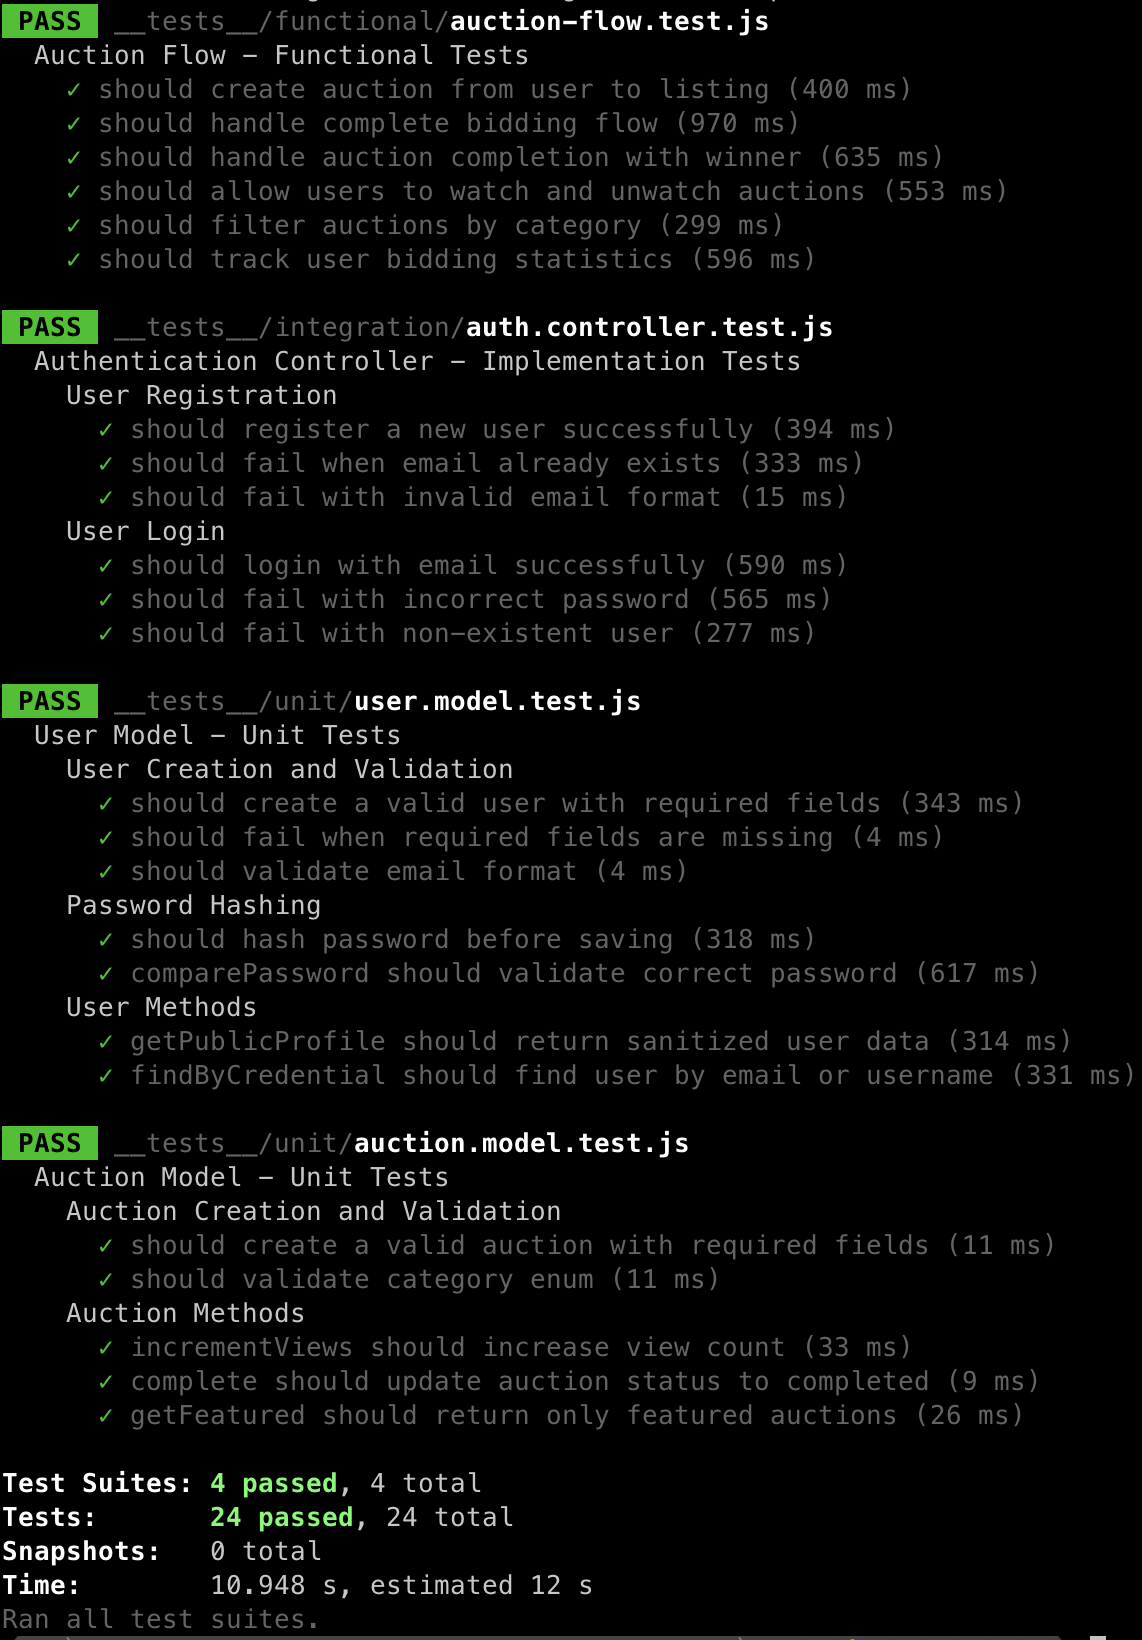
\includegraphics[width=\linewidth-130pt]{img/testy/testy.png}}
  \caption{Raport z uruchomienia testów systemu aukcyjnego}
  \label{fig:tutaj_tez_cos}
\end{figure}


